\documentclass{life-fr}
\usepackage{eurosans}
\usepackage{totpages}

\begin{document}

\title{Life is a Game}
\subtitle{Specification}
\member{Lepage Barbara}{db0company@gmail.com}
\member{Caradec Guillaume}{guillaume.caradec@gmail.com }
\member{El-Outmani Youssef}{youssef.eloutmani@gmail.com}
\member{Glorieux François}{fra.glorieux@gmail.com}
\member{Klarman Nicolas}{nickoas@gmail.com}
\member{Lassagne David}{david.lassagne@gmail.com}
\member{Le-Cor Wilfried}{wilfried.lecor@gmail.com}
\member{Lenormand Frank}{lenormf@gmail.com}
\member{Louvigny Guillaume}{guillaume@louvigny.fr}

\summary
{
  The specification aims to define just the "basic specifications" of our service work.
}

\maketitle

\chapter*{Abstract}
{
  This specification is a contractual document to define the specification of Life Is a Game, our EIP. \\
  It specifies the set of features, in addition to site architecture and mobile applications.\\
  The internal structure of the database will also be described.\\
  This document will also detail the potential targets of the project and attempt to estimate the financial and time constraints required to complete the implementation of this project.\\
  Finally the opening provided to third party developers will also be discussed.\\
}

\chapter*{Document Informations}

\begin{tabular}{ | m{5cm} | m{10cm} | }
  \hline
  Document Type & Specifications \\
  \hline
  Group Name & Life Is A Game \\
  \hline
  Number of pages & \ref{TotPages} \\
  \hline
  Full title of the document & Specifications Project `` Life Is A Game'' \\
  \hline
  Authors & Members of the group, see cover page \\
  \hline
  Manager & Group Leader: Barbara Lepage \\
  \hline
  Contact & lavieestunjeu@googlegroups.com \\
  \hline
  Keywords & `` specifications'','' `` lavieestunjeu \\
  \hline
  Current revision & 1.8 \\
  \hline
  Storefront & http://eip.epitech.eu/2014/lavieestunjeu/ \\
  \hline
  Not Available Official Website & \\
  \hline
\end{tabular}

\chapter*{Table of revisions}

\revision{1.0}{Lepage Barbara}{EIP Reminder}{05/04/2012}
\revision{1.1}{Louvigny Guillaume}{Basic principle for the future system}{05/04/2012}
\revision{1.2}{Lepage Barbara}{Hardware environment}{05/04/2012}
\revision{1.3}{Lenormand Frank}{Environment realizable}{05/04/2012}
\revision{1.4}{Lenormand Frank}{Technical Architecture}{05/04/2012}
\revision{1.5}{Klarman Nicolas}{Security Management}{05/04/2012}
\revision{1.6}{Lepage Barbara}{Sensitive points}{05/04/2012}
\revision{1.7}{Le-Cor Wilfried}{Description of the tests first level}{05/04/2012}
\revision{1.8}{Lassagne David}{Diagram of the database}{05/04/2012}
\listofrevisions

\newpage
\hspace{2cm}
\newpage

\tableofcontents

\newpage
\hspace{2cm}
\newpage

\chapter{EIP Reminder}
\section{What is an EIP and Epitech}

Epitech is providing an original formation to become an IT Expert. Always working on real projects, students learn to react and adapt their reactions depending of the situation for their future projects. For example, they will not be lost with technologies and languages they don’t know, they will just use the usual process they learn at school.

EIP means “Epitech Innovative Projects”. It is the most important step of Epitech studies. It started at the beginning of the third year and ended the last year. This project is achieved by a group of 6 students minimum. They work together for one goal : being innovative.
Moreover, the EIP show students the world of buisness.

\section{Subject of "Life is a Game"}

As part of our EIP we chose to create an entertaining social network based on bucket lists. A buck list is a list of ``things you want to do before dying'' : it define every things his author want to do of his life, a memo to not waste his life. Our project will let our visitors to make their own lists, validates their exploits, and let them publish these on other social networks. Thus, every action made by a user (adding an activity, success, failure) will be a conversation thread where his network and him would be able to discuss and share medias (photos, videos and so on). An user's activity will be validated by his own network, and will be shown as an achievement, like in video games. In the future the website will expand with other functionalities only existing in video games.

\newpage

\section{Basic principle for the future system}

Users targeted by the project are numerous. Just a person has an area of interest or passion cover (e) the site she has a reason to sign up. The site such as mobile applications are designed for an extended internationalization.\\

For end users the project will consist of a website and several mobile applications including Android, iOS and Windows Phone. For third party developers, an API will be created allowing the creation of new uses.\\

The EIP is designed to respond to a set of features not present in existing projects. These combined features are not present on the sites or competitors. Indeed, we wish to establish a platform playful enough to be visited daily, without neglecting the social aspect allowing visitors to discuss their leisure with its network easily and to share his experiences through pictures and videos.\\

After the first year of project work in partnership with INRIA and KOALAB Epitech, we believe we have a functional site. During the second year of work on the EIP we would like to sign commercial partnerships with various actors in cultural areas or events. This period will also be an opportunity to add new features appendices that meet needs eg from users.

\section{Goal of the project and recipients}

The project aims to create a user community around a system of "Achievements", directly related to everyday life, passions or professional life.\\

Targeted users are very numerous. In theory, anyone with a center of interest or passion is a target.\\

In the longer term, business partnership will target specific brands and locations.\\

The site will be multilingual, so open to internationalization.

\newpage

\section{What is an ``Achievement''?}

The term achievement (which can be translated as success or achievement in French) is, in part videogame, set a goal to be accomplished by the player, outside the main objective (that is to say, win or finish the game).\\
The Achievements are honorary awards adding challenge for the player.\\
\\
We could use a French translation of the term achievement but we believe that achievement is the term most popular worldwide video-fun.\\
\\
The Achievements allow the player to explore more deeply the game content and therefore to explore new horizons.\\
The achievement is often a good time for the player.\\
He feels a certain satisfaction and feels rewarded for the effort.\\
It can then share with his friends to collect the honors or challenge their friends to do the same or better, which greatly improves the immersion in the game \\
\\
We believe, it is interesting to draw an analogy with life.\\
Life is a game like any other and is also deserves its Achievements.\\

\section{Technological context}

Today the one hand increasingly important Internet users are equipped with smartphones, it is even provided that the number of users exceeds the mobility of users settled within a few years.\\
\\
To adapt to this change and cope with the significant expansion of new technologies, we chose to offer our users of versions dedicated to major mobile platforms.\\
\\

\newpage
\hspace{2cm}
\newpage


\chapter{Introduction to Environmental realizable}

\section{Hardware Environment}

Our project runs on a server Ocsigen. It is installed on a Dell PRO Dedibox funded by project members.

\vspace{20pt}

\begin{tabular}{|c|c|}
  \hline
   Server & Dell® PowerEdge R210\\
  \hline
  Processor & 1x Intel® Xeon® L3426\\
  \hline
  Architecture & 4x 1.86GHz, 64 Bits, Virtualization\\
  \hline
  RAM & 16 Go DDR3 ECC\\
  \hline
  HDD & 2 x 2 To SATA2 Raid 0 / Raid 1 HARD (H200)\\
  \hline
  Monthly price & 49,99 euros HT\\
  \hline
\end{tabular}

\vspace{20pt}

\section{Costs}

\begin{itemize}
  \item A developer account for each store application (IOS: AppStore (99 \$), Play Google (Android: 25 \$) and Windows Phone Marketplace (99 \$)) for mobile applications.
  \item A dedicated server, initially built for the development of the site can handle only a few users connected simultaneously at about 60 euros per month.
  \item A production server, which will later be used up to 600 euros per month.
  \item We see later, once the application is fully completed, to hire a graphic designer for "Achievements".
\end{itemize}

\newpage

\section{Realization Environment}

To communicate and discuss the project, our working group relies on several tools.

\begin{itemize}
  \item Indeed, Life Is A Game has its official IRC channel (\# irc.epitech.net on life-eip), whose goal is to provide quick support to users and contributors by managing a chat history.
  \item Additionally, the project team has access to a mailing list (hosted by google groups).
  \item It manages all documents relating to the project's progress through google documents.
  \item Documentation can be found on the showcase site: \url {http://eip.epitech.eu/2014/lavieestunjeu/}
  \item We have a bug tracker, wiki and tickets to a private GitHub repository.
\end{itemize}

\section{Technical Architecture}

\begin{itemize}
  \item Life Is A Game is based on a Web environment in OCaml, so the main component is the web server \href{http://ocsigen.org/}{Ocsigen}.
  \item The project will also build on \href {http://ocsigen.org/js_of_ocaml/}{js \_of \_ocaml}, a tool for compiling OCaml JavaScript.
  \item It will manage a database using \href {http://ocsigen.org/macaque/}{Macaque}, another project initiated by INRIA.
\end{itemize}

\section{Security Management}

\begin{itemize}
  \item Implementation of a solution of "privacy level", a user can define a level of privacy for each user on its network.

\begin{figure}[H]
  \begin{center}
    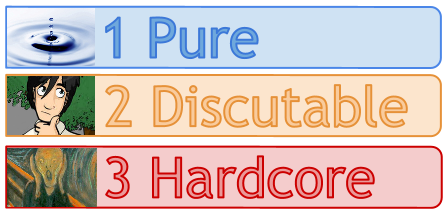
\includegraphics[width=10cm]{img/confidentialite.png}
  \end{center}
\end{figure}

\end{itemize}

\section{Sensitive points}

\begin{itemize}
  \item Information security is a priority for us. We will therefore pay close attention to what users are always aware at any time who has access to what information.
  \item We want to keep our ideas secret until we have a basic version available.
\end{itemize}

\chapter{Description of the different parts of the program to make}

\section{The Website}

\subsection{Overview of the homepage before login}

The user will see first a slide show highlighting some "Achievements", arranged by date of publication and popularity, and the various functions of the site. This slide show will aim to encourage the user to carry their registration.\\

The home page will also allow the user to register with the site. This registration is detailed below.\\

The last main feature of this home page is the user login to the site.\\

The entrance to the site could eventually help to find the "Achievements" and categories of the latter.

\newpage

\subsection{The subscription, the first five minutes!}

The objective of this step is clearly to avoid the cumbersome that represents the collection of information that the site needs to do with the future user (present a compact form and wild is likely to discard it and possibly to do surrender its registration).\\

So we thought of a system in which single-step mode, while our tool and discover her world to the user, it would make subtle inquiries on a regular basis, in order to alleviate this essential step allow us to categorize the new registrant and to offer content based on these information have been collected.\\

In addition to combining the role of "guide" for the discovery of the site and "Sounder" for information gathering, this method has the advantage of pushing the user to go after the presentation, and thus the registration, as and when the group advanced (psychological effect, he wants to finish what he started, having already begun to contribute as well go all the way). The presentation from the growing interest, the chances increase of a registration upon arrival.\\
\\

In the present state we can imagine as a first approach a simple question that leads to a single action mode "you are one click to enter our universe" with, for example, the choice of gender: Male, Female, Not stated .

\begin{figure}[H]
  \begin{center}
    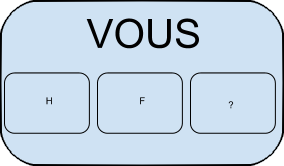
\includegraphics[width=10cm]{img/vous.png}
  \end{center}
\end{figure}

\newpage

\subsection{The user home page once logged}

The home page of the user used the site presents its information flow, like the usual stream sites such as Facebook or Google +. \\

The menu must be discreet. The user should immediately see the four main tabs:

\begin{itemize}
  \item Feed (default homepage);
  \item the user's objectives;
  \item "Achievements";
  \item "friends" of the user (or imported from social networks within the site).
\end{itemize}

A bar of "breaking news" constantly on top of the site will give the user the latest in a line "Achievements" to his friends and the new homepage.

\begin{figure}[H]
  \begin{center}
    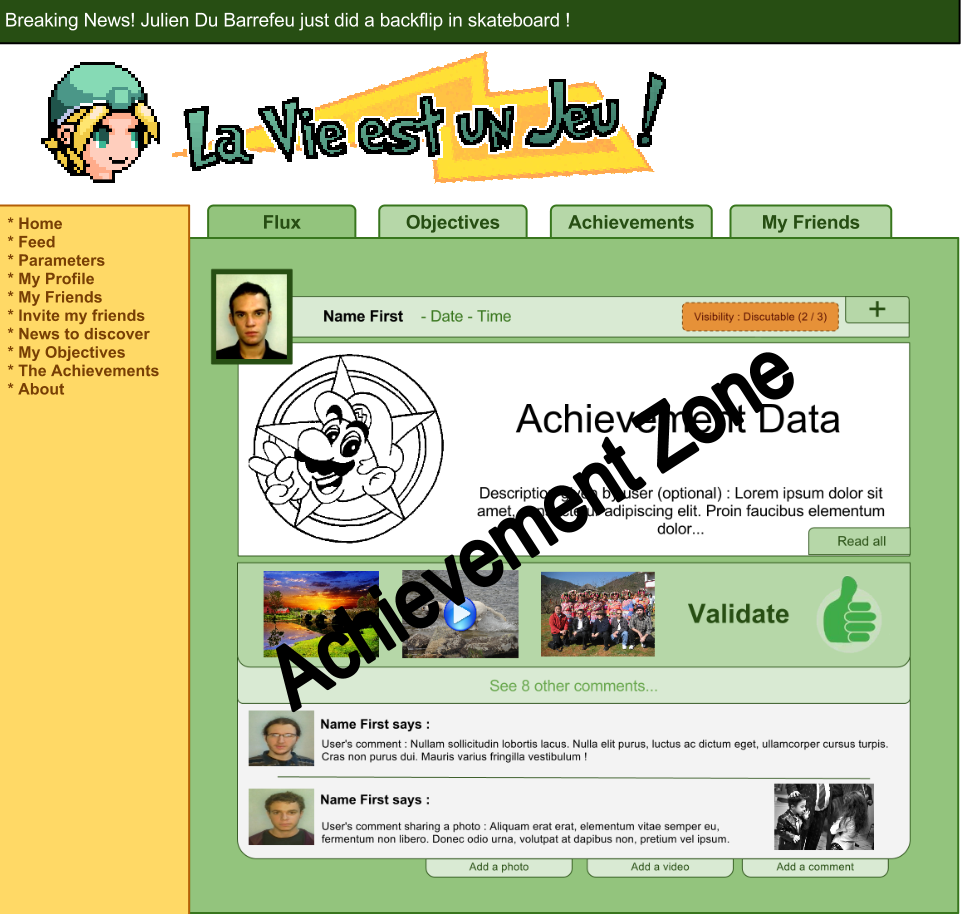
\includegraphics[width=15cm]{img/accueil.png}
  \end{center}
\end{figure}


\subsection{Feed tab}

The feed tab will be located in the middle of the main page and will feature displays the most recent "Achievements" to be validated by the circle of friends.\\

This feed will contain all the actions of contacts:

\begin{itemize}
  \item "Achievements" to validate (see details below);
  \item the goals they set for themselves;
  \item new contacts;
  \item new on the site (or new information "Achievements").
\end{itemize}

\newpage

\subsection{Achievements details}

Each "achievement" will have a Like feature that will allow users to indicate they like the publication in question, and a sending module evidence of "Achievements" for validation. The validation support can be text, photo or video. The user's photo will appear as the description of "achievement", next to it. It will also be possible to post comments below evidence of validation. A tab "More" will take place every "achievement" to get more information.\\

\begin{figure}[H]
  \begin{center}
    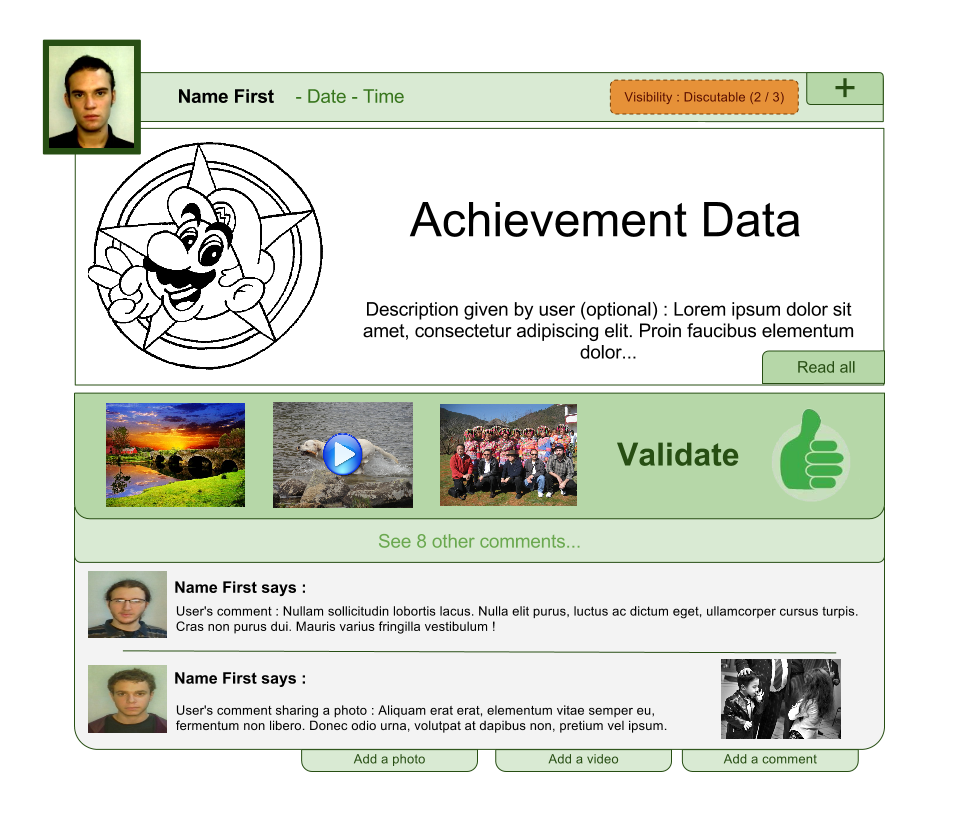
\includegraphics[width=15cm]{img/achievement.png}
  \end{center}
\end{figure}

\subsection{Achievements tab}

The user can select packages that contain the "Achievements" to accomplish. The packs will be available all classified by theme and in a subcategory, but the platform will provide the user first packages of "Achievements" corresponding to the interests of the latter, or its edge of age. Once a package is selected, the user can also define some "Achievements" as its objectives, and so notify its network.

\newpage

\subsection{Objectives tab}

The Objectives tab allows the user to build a "to-do list" or "bucket list", in order to filter the "Achievements" that the user does not wish to make an immediate and so clear those he will accomplish in the short term. The page is intended to be regularly consulted: it is from this tab the user can announce the end of a goal, and thus obtain an "achievement" if his friends confirm the validation of the latter.

\subsection{Contacts tab}

The user can see here their contact list and profiles of these, but also group contacts by group. User groups can then assign degrees of sensitivity.
The sensitivity ranges from 0 to 3 and to share the "Achievements" to contacts of their choice.

\subsection{Profile page}

The Profile page contains information of a user, and can change them. If the user is viewing the profile page of another member, he has the opportunity to interact with it in different ways (sending a message, request to add a friend, ...).
The profile page contains mainly badges "achievement" as a hunting scene. The user can click on the "achievement" for the full (text, photos, videos, comments).

\section{Smartphone Apps}

As for smartphones, we decided not to code in languages specific to each platform, but to develop an interface based on the technology we use for our website, namely Ocsigen. This will allow us to be consistent in our guideline of code. This interface will be charged on all smartphone platforms in the form of a web-view. The advantage of this method lies in its total portability that we do not have to develop an application specific to each existing platform.

\section{API}

The API would provide developers access to the essential features of the site. We can come back, for a given user, and according to the wishes of the latter (token of acceptance), the list of "Achievements".

\chapter{Databases description}

\section{First levels tests}

\begin{itemize}
  \item Account Creation
  \item Access restriction by circles
  \item listing of "Achievements" already present in the database.
  \item Selection of "Achievements" from those available.
  \item Weighting "Achievements".
  \item classification: tests of different scoring algorithms.
  \item Restriction of the achievements for a class of users (those at level 3 will not be available at least 18 years of age and those at Level 2 under 14).
\end{itemize}

\section{Outline of the database}

\begin{figure}[H]
  \begin{center}
    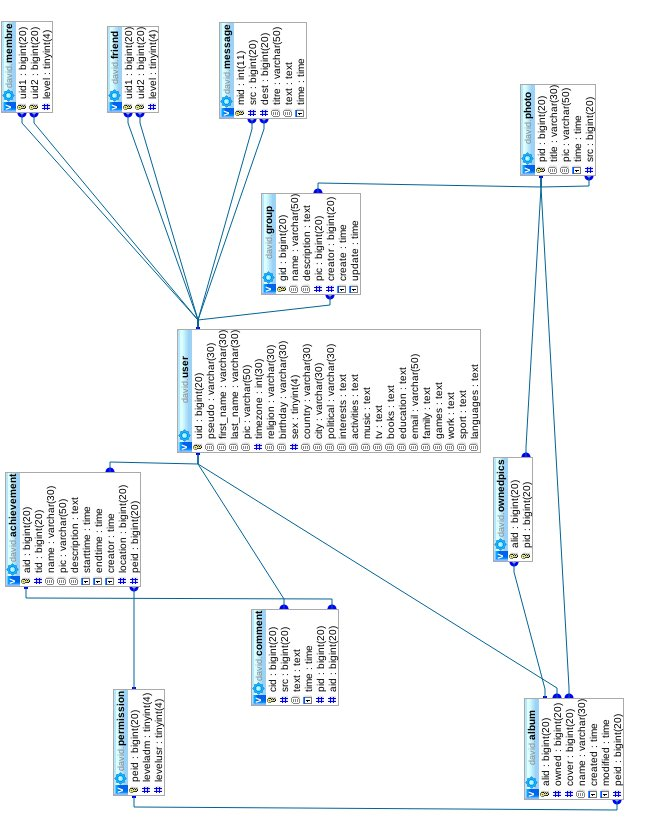
\includegraphics[width=18cm]{img/imgdb.jpg}
  \end{center}
\end{figure}

\chapter{Project Organization}

\section{Planning}

From a global perspective, the project will proceed in three main sections: documentation, development and production.\\

Before turning to the concrete realization of the product, we will devote ourselves to the drafting of several key documents to the project runs smoothly. Indeed, it is necessary to precisely define the details of the project, study the various tools and technologies at our disposal and make choices, or develop partnerships. We will continue this study until September 2012.\\

Once the tools at hand, the specific and defined roles, we will begin to develop the product. We expect to release a beta version in September 2013.\\

The last period will be devoted to communication issues, and to a lesser degree of development. Thus, during the last year of the project, we will try to express it in various ways to create community is indispensable to our platform, in addition to the finalization of the technical product. We can thus benefit from user feedback in order to correct anomalies and refine the platform.

\newpage

\section{Team}

During the product development team will be dispersed in several countries, making any teamwork difficult. We will allocate tasks so as to be able to work relatively autonomously: our project is composed of several distinct elements, we will arrange to not share one between members located in different places.\\

At the division of roles: Guillaume Caradec handles project management, and Barbara Lepage directs the technical part. We are obviously all the responsibility of developing and writing documentation.\\

We have at our disposal various tools to get organized and communicate more easily: \\

\begin{itemize}
  \item a mailing list and an IRC channel, to treat all the various issues;
  \item a Google Docs file, so you can share documents related to the project and writing;
  \item Gtalk, Google's application for organizing video conferences via a browser;
  \item a Git;
  \item using Doodle to schedule meetings more easily.
\end{itemize}

Group members will meet weekly to discuss project progress, and unanticipated set of short-term goals.

\section{Detailed schedule with specific dates}

Please see the attached file \texttt {2014\_GAN\_EN\_lavieestunjeu.pdf}. It contains the Gantt chart of our project.


\newpage
\hspace{2cm}
\newpage


\chapter{Conclusion}

This paper presented the specification so our EIP, Life Is a Game \\
\\
We have described all the features that will be proposed, which includes both the website and mobile applications.\\
\\
Was also presented the definition of the database on all applicable platforms covered.\\
\\
The API destined for third-party developers had also been defined.\\
\\
Finally, he detailed also those who can win the project, and estimated the various constraints imposed by it be they financial or organizational.\\

\newpage
\hspace{2cm}
\newpage

\chapter {Appendix}

\section {Glossary}

\subsection {Algorithm}

And finite sequence of unambiguous instructions to give the answer to a problem.

\subsection {API}

Programming Interface, it is an interface provided by a computer program for the interaction of programs with each other.

\subsection {Mobile Application}

A mobile application is an application developed to be installed on mobile electronic devices.

\subsection {Web Architecture}

Web-based architecture means the general structure inherent in a web environment.

\subsection {Database}

A database is a lot of information stored in a computing device.

\subsection {bug tracker}

`` Software'' issue tracking, software to help users and developers to improve software quality by finding the flaws of such software.

\subsection {Specification}

Specification is to simply define the specifications of a product or service to achieve.

\subsection {Repository}

A repository is a centralized storage and organizing data.

\subsection {Gantt Chart}

A Gantt chart is a tool used in scheduling and project management and for viewing in time the various tasks a project component.

\subsection {Slideshow}

A slideshow is a sequence of images or documents connected by and effects on which it is possible to sound.

\subsection {Doodle}

Doodle.com is a website planning and survey of the Swiss company Doodle AG.

\subsection {GitHub}

Github is a Web service hosting and management of software development, Git using the program. 

\subsection {Google Docs}

Google Docs is a result of changes in Google Spreadsheets, word processing software. These programs allow a merged online collaboration.

\subsection {Google Talk}

Google Talk is proprietary software and instant messaging service and VoIP Jabber-based and developed by Google.

\subsection {IRC}

IRC is a protocol text communication on the internet.

\subsection {JavaScript}

JavaScript is a scripting programming language used primarily for interactive web pages.

\subsection {Login}

`` ID'', information enabling a person to identify themselves to a system.

\subsection {Mailing List}

Specific use of electronic mail that allows direct mail information to users who are enrolled.

\subsection {Production start}

Provision `` total'' of a service or product.

\subsection {Ocaml}

Formerly known as Objective Caml is the most advanced implementation of Caml programming language.

\subsection {Ocsigen}

Web development framework, developed by the French laboratory PPS.

\subsection {Network}

Mesh of links between different computer equipment allowing sharing of information.

\subsection {social network}

Set of social identities, such as individuals or organizations linked together by bonds created during social interactions.

\subsection {Service}

Adds value to a product or work required to ensure a company or an individual.

\subsection {storefront}

Website composed of a few pages with a company. Allows a company to communicate with the world.

\subsection {Smartphone}

With mobile phone also features a PDA. It provides basic functionality such as calendar, calendar, web browsing, consulting e-mail, instant messaging, GPS ...

\subsection {Android}

Operating system using the Linux kernel for smartphones, mobile PDAet designed by Android, a startup acquired by Google.

\subsection {IOS}

Mobile operating system developed by Apple for iPhone, iPod touch, and the iPad. It is derived from Mac OS X with which it shares foundations.

\subsection {Windows Phone}

Mobile operating system developed by Microsoft as the successor to Windows Mobile, its previous software platform.

\subsection {Beta}

Test version includes all the features of a program. It is through this version that testers back any problems.

\subsection {Wiki}

Collaborative space where users are invited to write papers.

\newpage
\hspace{2cm}
\newpage

\end{document}
